\chapter{Discussion}\label{chp.discussion}

As indicated in Section~\ref{chp.Criticism.Readers}, many readers see the rise of other-direction type at the expense of inner-direction type and therefore, lose the hopes and be pessimistic to the society. Thereafter, it is also important to reiterate that other-direction is not necessarily a bad thing, mainly discussed in~\ref{chp.reinterpretation}. What really matters is that we should be aware of its pull, so that being able to transcend and rise above it instead of letting it dominate our lives. Only by understanding something, one could free himself from it. Therefore, from this position of freedom and autonomy, the autonomous type of person is introduced, who is able to choose when to conform and when to resist.\\

As indicated in~\ref{chp.solution}, it is worth striving for the autonomous type, benefiting not only ourselves but also influencing the society and the next transition in the future. However, there are many challenges to become a autonomous person in this other-directed age. In this chapter two challenges are mainly introduced, namely the impact of the anxiety of the other-directed people and the impact of the mass media.\\

\textbf{Impact of the anxiety}
As indicated in Section~\ref{chp.reinterpretation.cost}, while striving for autonomous, we are suffering from a new form of anxiety about what to do and whom to trust. On one hand, the anxiety comes from the uncertain choice due to the large amounts of consuming possibilities. As is suggested by~\citeauthor{bude2014gesellschaft}, this anxiety, stem from the fear, could be defined as the feeling of helpless when we face the uncertainly, which is not derived so much from a ``powerful other'' but rather from the seemingly endless range of possibilities we face~\citep{bude2014gesellschaft}. One the other hand, as indicated in Section~\ref{chp.reinterpretation.cost}, other-directed people tend to compare their own experiences with different experiences that others are having, resulting in the uncertainty about whether the choice they made are properly. In order to reduce the impact of such anxiety, it is important to have confidence in ourselves, especially in making the choices, namely, instead of spending time comparing with others, we should also take the time listening to the inner voice and making our own choice, which follows the heart. Moreover, we should also be brave enough to do what we thought is appropriate, even it is different from what others normally do, since the society needs pioneers instead of followers.


%``Anxiety springs from the knowledge that everything is open but nothing is meaningless,'' he wrote, ``Our entire lives seem to be on the line at every single moment. The fear of simply drifting through life is hard to bear''. Every single ``wrong'' choice, such as choosing the ``wrong'' school, a ``wrong'' person to marry, could lead to the ``failure'' of life. We are struggling from the threat of the negative results instead of striving for success~\citep{bude2014gesellschaft}.

\textbf{Impact of The Mass Media}
Newspapers, books, magazines, comics, television, radio, movies, records, video games and the Internet, MP3 players, and smart phones, are all examples of what sociologists refer to as mass media--forms of a communication that reach a large audience. 

It is well-known that the media has literally become part of our everyday environment and is much more powerful and widespread than we thought, since the reach of the mass media has become so extensive, diverse and constant that it is difficult to find any person or any place in the world that does not have some regular exposure to media on daily basis~\citep{callero2017myth} and the society is more and more dominated by commerce and news. (refers to the Figure~\ref{discussion.fig.media})

\begin{figure}{t!}
  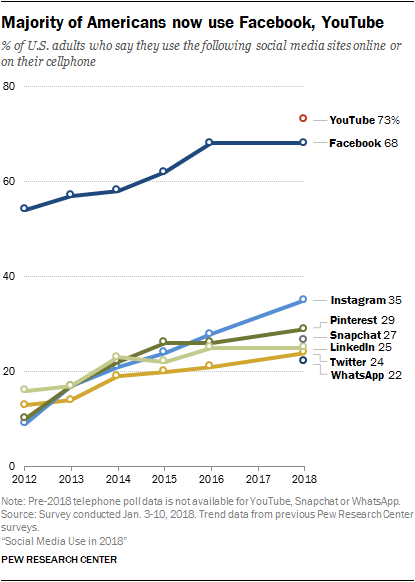
\includegraphics[width=\linewidth]{mass_media.png}
  \caption{The increase of the usage of the different kinds of social networks in the USA}
  \label{discussion.fig.media}
\end{figure}

Many worried about its threat to the individualism, since the other-directed people could easily be influenced by the mass media. Also written by David Riesman in the preface of the book ``The Lonely Crowd'', the gravest concern of the authors about the mass media, however, is not their long-run impact on culture, but the fact that the press, the news, the magazines, and particularly the newsreels have become far more ethnocentric and less parochial, which somewhat cover more foreign news, and only to smother it in the self-serving slogans and misleading the crowd. Edward W. Said also suggested that, ``despite the variety and the differences, and however much we proclaim the contrary, what the media produce is neither spontaneous nor completely ``free'': ``news'' does not just happen, pictures and ideas do not merely spring from reality into our eyes and minds, truth is not directly available, we do not have unrestrained variety at our disposal.'' In this information-saturated world, where the information could be both helpful and misleading, we need all the information we can get about all the information we are receiving and need to learn to pick the information we need and worth trusting, meanwhile, to be aware of the faking possibilities and think critical. 
% For example, as the online shopping is very popular and convenient, the ratings and reviews for a good are more and more important for the customers, which is also known by the sellers. Thereafter, they hire someone to rate the product high and write recommendations and compliments for the product, though it works not the same as is described. One one hand, the rating and reviewing system could help us to decide which to buy, on the other hand, some fake and misleading information may lead to the waste of money and time. 






 


			



